\section*{Supplementary Materials}
\renewcommand\thefigure{S\arabic{figure}}
\renewcommand\theequation{S\arabic{equation}}
\setcounter{figure}{0}
\setcounter{equation}{0}

\subsection*{A compartmental model for asymptomatic/symptomatic cases}

Consider an SEIR model variant in which an infected individual can be either asymptomatic, $I_a$, or symptomatic, $I_s$.
We note that $I_a$ and $I_s$ represent prevalence (i.e., the total number of currently infectious individuals) of asymptomatic and symptomatic individuals; these quantities are different from $i_s$ and $i_s$ that we present in the main text, which represent incidence (i.e., the rate at which new cases are generated)  of asymptomatic and symptomatic individuals.
While both cases can recover, we assume that only symptomatic cases can lead to fatalities, denoted
by the $D$ category.
In total, the dynamics of susceptibles, exposed, infectious, recovered, and dead are:
\begin{eqnarray}
\dot{S}&=&-\beta_a S I_a -\beta_s S I_s \\
\dot{E}&=&\beta_a S I_a +\beta_s S I_s -\gamma_e E\\
\dot{I}_a&=&p\gamma_e E-\gamma_a I_a\\
\dot{I}_s&=&(1-p)\gamma_e E-\gamma_s I_s\\
\dot{R}&=&\gamma_a I_a + (1-f)\gamma_s I_s \\
\dot{D}&=&f\gamma_s I_s.
\end{eqnarray}
Here, $\beta_a$ and $\beta_s$ denote transmission rates,
$\gamma_e$ denotes the transition from exposed to infectious,
$p$ is the fraction of asymptomatic cases that
are generated for each exposed individual,
$1-p$ is the fraction of symptomatic cases that
are generated for each exposed individual,
$\gamma_a$ and $\gamma_s$ denote recovery rates,
and $f$ denotes the case fatality ratio for symptomatic cases.

Given that the number of infected individuals increase exponentially at rate $r$ initially, the equations
for the infectious cases can be rewritten given the ansatz
$E(t)=c_e e^{rt}$,
$I_a(t)=c_a e^{rt}$,
$I_s(t)=c_s e^{rt}$.
Then, it follows that 
\begin{eqnarray}
r c_a&=&p\gamma_e c_e-\gamma_a c_a,\\
r c_s&=&(1-p)\gamma_e c_e-\gamma_s c_s,
\end{eqnarray} 
which implies that
\begin{equation}
\frac{c_a}{c_s}=\frac{p}{1-p}\left[\frac{r+\gamma_s}{r+\gamma_a}\right].
\end{equation}
The prevalence of asymptomatic and symptomatic individuals is different from $p$ and $1-p$ because prevalence measures the individuals that are currently infectious and does not account for individuals that have already recovered.
Finally, the ratio of secondary case production caused by asymptomatic vs.~symptomatic
individuals during the exponential phase should be
\begin{equation}
\frac{q}{1-q} = \left(\frac{\beta_a}{\beta_s}\right)\frac{p}{1-p}\left[\frac{r+\gamma_s}{r+\gamma_a}\right],
\end{equation}
where $q$ is the fraction of new secondary cases caused by
asymptomatic individuals.

The basic reproduction number of this system is:
\begin{equation}
{\cal{R}}_{0}= p {\cal{R}}_a + (1-p) {\cal{R}}_s,
\end{equation}
where 
\begin{eqnarray}
{\cal{R}}_a &=& \frac{\beta_a}{\gamma_a},\\
{\cal{R}}_s &=& \frac{\beta_s}{\gamma_s}.
\end{eqnarray}
The generation-interval distributions for asymptomatic and symptomatic individuals follow the same functional form as the corresponding generation-interval distribution for a single-type SEIR model since both asymptomatic and symptomatic individuals have exponentially distributed latent and infectious periods \citep{svensson2015influence}:
\begin{eqnarray}
g_a(\tau) &=& \frac{\gamma_e \gamma_a}{\gamma_e - \gamma_a} \left(\exp(-\gamma_a \tau) - \exp(-\gamma_e \tau)\right),\\
g_s(\tau) &=& \frac{\gamma_e \gamma_s}{\gamma_e - \gamma_s} \left(\exp(-\gamma_s \tau) - \exp(-\gamma_e \tau)\right).
\end{eqnarray}
It immediately follows that 
\begin{equation}
\left(\frac{z}{1-z}\right)\left[\frac{\int_0^\infty \exp(-r\tau) g_a(\tau) \mathrm{d}\tau}{\int_0^\infty \exp(-r\tau) g_s(\tau) \mathrm{d}\tau}\right] = \left(\frac{\beta_a}{\beta_s}\right)\frac{p}{1-p}\left[\frac{r+\gamma_s}{r+\gamma_a}\right],
\end{equation}
where $z = p {\cal{R}}_a/{\cal{R}}_{0}$ and $1-z=(1-p) {\cal{R}}_s/{\cal{R}}_{0}$.

\pagebreak

\subsection*{Supplementary figures}

\begin{figure*}[!ht]
\begin{center}
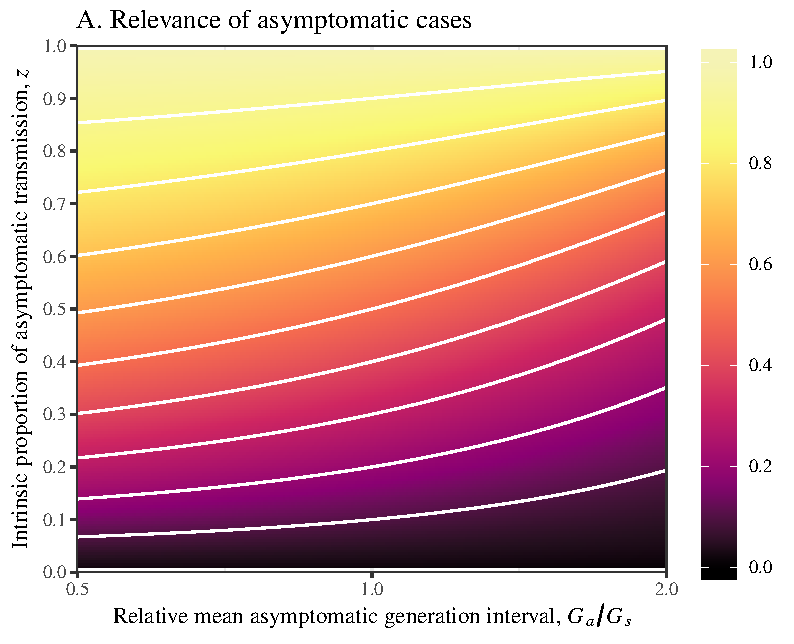
\includegraphics[width=0.4\textwidth]{figheatmap_03.pdf}
\mbox{\hspace{0.05\textwidth}}
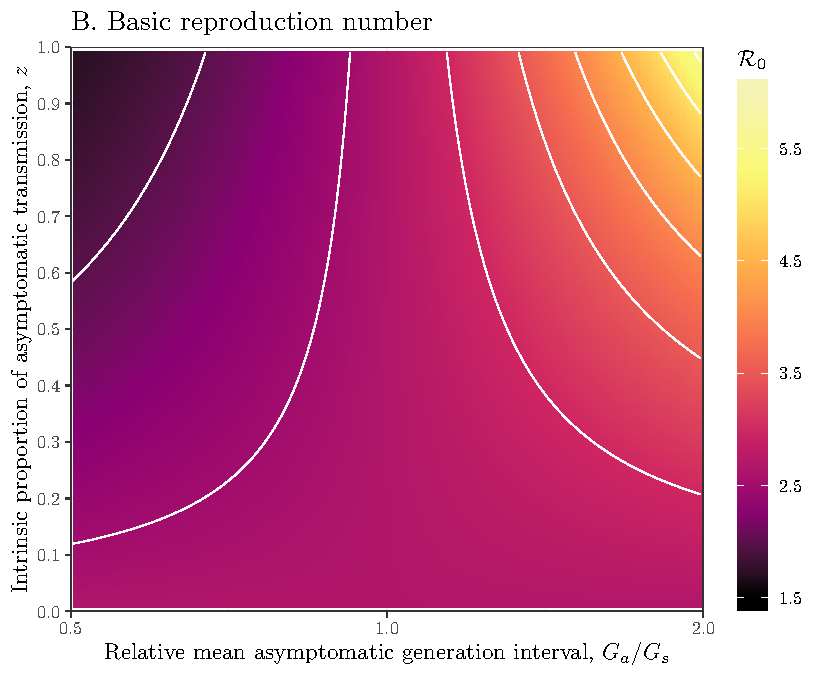
\includegraphics[width=0.4\textwidth]{figheatmap_R0_03.pdf}
\caption{Effects of intrinsic proportion of asymptomatic transmission on the relevance of asymptomatic transmission and basic reproduction number, given variation in
the mean generation interval of asymptomatic cases when generation-interval distributions are narrow. 
We vary $G_a/G_s$ while assuming $1/r=7$ days, $\bar G_s=8$ days, and $\kappa_s=\kappa_a=0.3$.
See Figure 1 in the main text for figure caption.
}
\end{center}
\end{figure*}

\pagebreak

\begin{figure*}[!ht]
\begin{center}
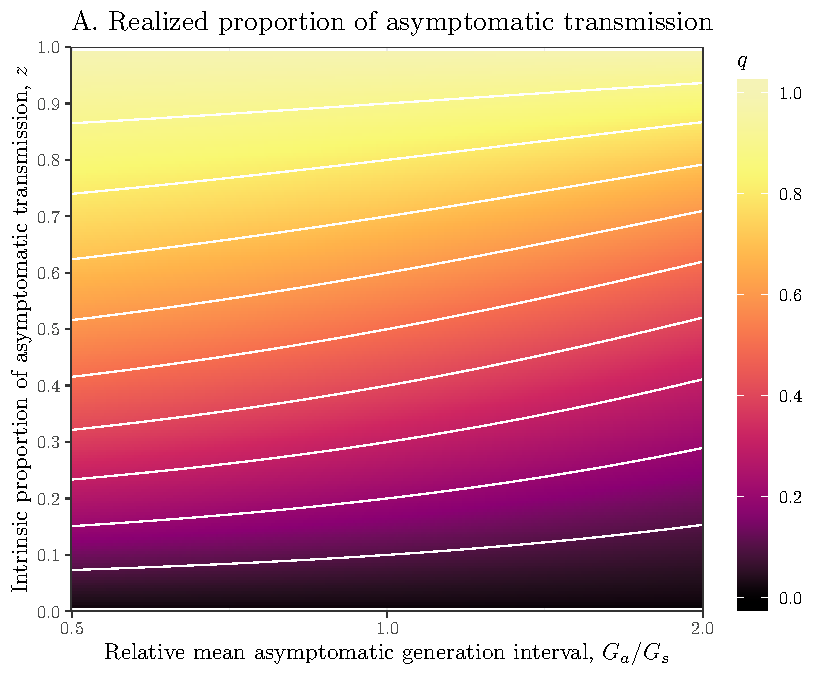
\includegraphics[width=0.4\textwidth]{figheatmap_08.pdf}
\mbox{\hspace{0.05\textwidth}}
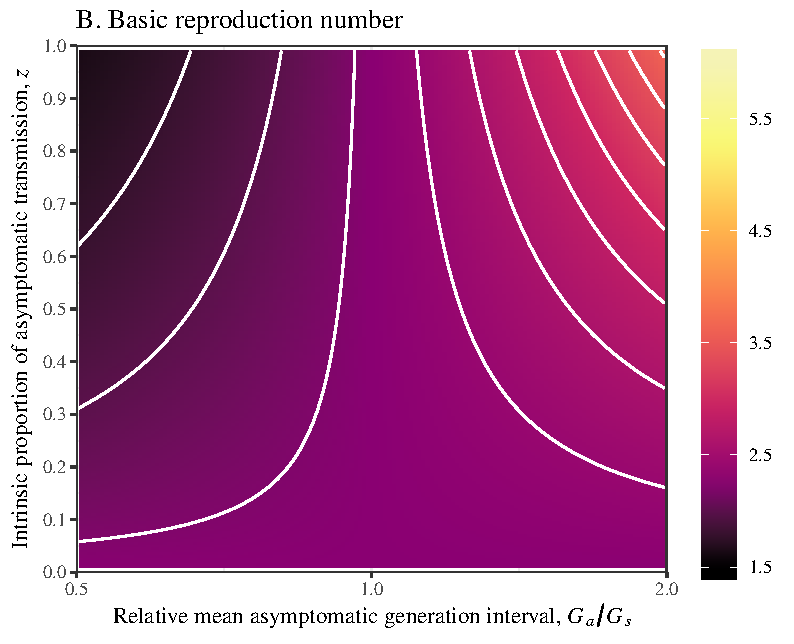
\includegraphics[width=0.4\textwidth]{figheatmap_R0_08.pdf}
\caption{Effects of intrinsic proportion of asymptomatic transmission on the relevance of asymptomatic transmission and basic reproduction number, given variation in
the mean generation interval of asymptomatic cases when generation-interval distributions are wide. 
We vary $G_a/G_s$ while assuming $1/r=7$ days, $\bar G_s=8$ days, and $\kappa_s=\kappa_a=0.8$.
See Figure 1 in the main text for figure caption.
}
\end{center}
\end{figure*}

\pagebreak

\begin{figure*}[!ht]
\begin{center}
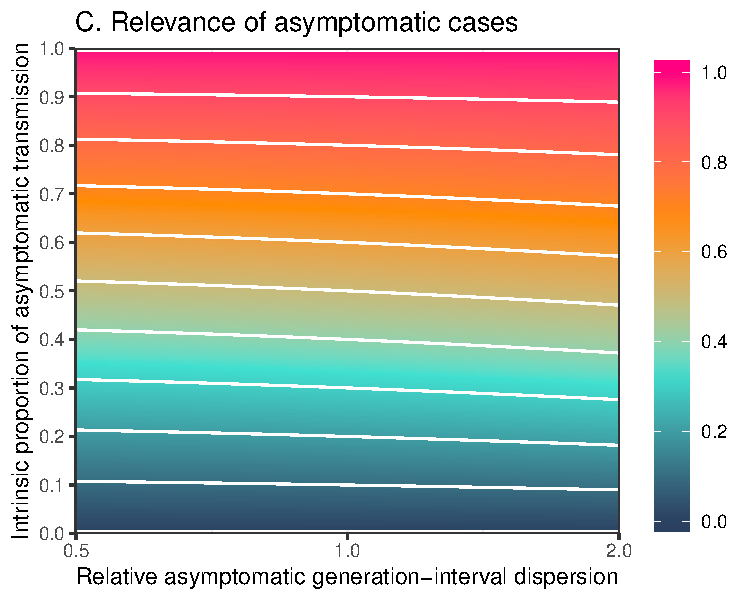
\includegraphics[width=0.4\textwidth]{figheatmap_kappa.pdf}
\mbox{\hspace{0.05\textwidth}}
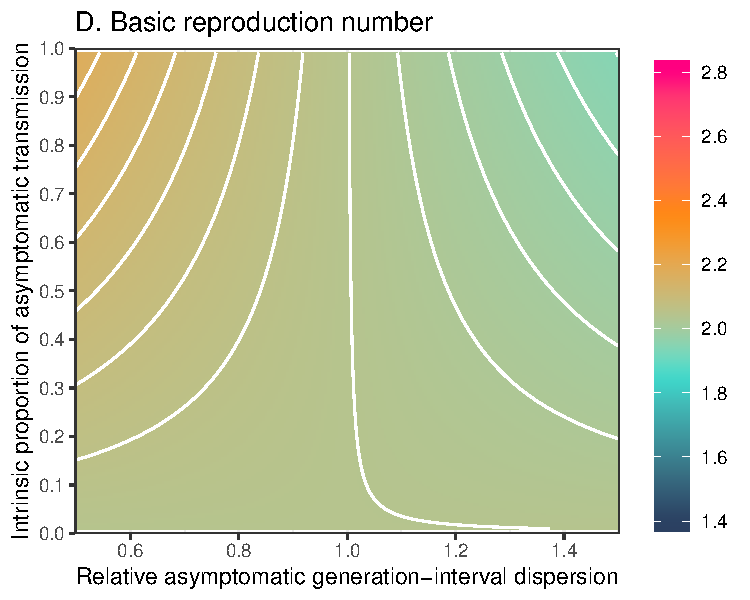
\includegraphics[width=0.4\textwidth]{figheatmap_kappa_R0.pdf}
\caption{Effects of intrinsic proportion of asymptomatic transmission on the relevance of asymptomatic transmission and basic reproduction number, given variation in
the generation-interval dispersion of asymptomatic cases.
(A) Wide/narrow generation intervals of asymptomatic cases increase/decrease the relevance of asymptomatic cases, $q$.
(B) Wide/narrow generation intervals of asymptomatic cases decrease/increase the basic reproduction number ${\cal{R}}_0$.
We vary $\kappa_a/\kappa_s$ while assuming $1/r=7$ days, $\bar G_s=\bar G_a=8$ days, and $\kappa_s=0.5$.
The white lines represent the contours.
}
\end{center}
\end{figure*}

